% This is text associated with the open textbook "Open Electromagnetics"
% See immediately below for author, date
% This work is licensed under the Creative Commons Attribution-ShareAlike 4.0 International License. (CC BY-SA 4.0) 
% To view a copy of the license, visit http://creativecommons.org/licenses/by-sa/4.0/

%ORB TITLE Current Distributions
%ORB AUTHOR 0        # S.W. Ellingson, Virginia Tech (ellingson@vt.edu)
%ORB DATE 20180806   # yyyymmdd
%ORB ABSTRACT Current Distributions 

\label{m0101_Current_Distributions} % <-- Must match name of this file and module directory name.  Don't mess with this!
\index{current density|(}

In elementary electric circuit theory, current is the rate at which electric charge passes a particular point in a circuit. For example, 1~A is 1~C per second.
In this view current is a scalar quantity, and there are only two possible directions because charge is constrained to flow along defined channels.
Direction is identified by the sign of the current with respect to a reference direction, which is in turn defined with respect to a reference voltage polarity.
The convention in electrical engineering defines positive current as the flow of positive charge into the positive voltage terminal of a passive device such as a resistor, capacitor, or inductor.
For an active device such as a battery, positive current corresponds to the flow of positive charge \emph{out of} the positive voltage terminal.

However, this kind of thinking only holds up when the systems being considered are well-described as ``lumped'' devices connected by infinitesimally thin, filament-like connections representing wires and circuit board traces.
Many important problems in electrical engineering concern situations in which the flow of current is not limited in this way. Examples include wire- and pin-type interconnects at radio frequencies, circuit board and enclosure grounding, and physical phenomena such as lightning.
To accommodate the more general class of problems, we must define current as a vector quantity.
Furthermore, current in these problems can spread out over surfaces and within volumes, so we must also consider \emph{spatial distributions} of current.  

{\bf Line Current.}
\index{current density!line}
As noted above, if a current $I$ is constrained to follow a particular path, then the only other consideration is direction.  Thus, a line current is specified mathematically as $\hat{\bf l}I$, where the direction $\hat{\bf l}$ may vary with position along the path.
For example, in a straight wire $\hat{\bf l}$ is constant, whereas in a coil $\hat{\bf l}$ varies with position along the coil.

{\bf Surface Current Distribution.} 
\index{current density!surface}
In some cases, current may be distributed over a surface.
For example, the radio-frequency current on a wire of radius $a$ made from a metal with sufficiently high conductivity can be modeled as a uniform surface current existing on the wire surface.  
In this case, the current is best described as a surface current density ${\bf J}_s$, which is the total current $I$ on the wire divided by the circumference $2\pi a$ of the wire:
%
\begin{equation}
{\bf J}_s = \hat{\bf u}\frac{I}{2\pi a}~~\mbox{(units of A/m)}
\end{equation} 
%
where $\hat{\bf u}$ is the direction of current flow. 

{\bf Volume Current Distribution.} 
\index{current density!volume}
Imagine that current is distributed within a volume.   
Let $\hat{\bf u}\Delta i$ be the current passing through a small open planar surface defined within this volume, and let $\Delta s$ be the area of this surface.
The \emph{volume current density} ${\bf J}$ at any point in the volume is defined as
%
\begin{equation}
{\bf J} \triangleq \lim_{\Delta s \to 0} \frac{\hat{\bf u}\Delta i}{\Delta s} = \hat{\bf u}\frac{di}{ds}~~\mbox{(units of A/m$^2$)}
\end{equation}
%
In general, ${\bf J}$ is a function of position within this volume.
Subsequently the total current passing through a surface ${\mathcal S}$ is
%
\begin{equation}
I = \int_{\mathcal S} {\bf J}\cdot~d{\bf s}~~\mbox{(units of A)}
\end{equation}
%
In other words, volume current density integrated over a surface yields total current through that surface.  
You might recognize this as a calculation of flux, 
\index{flux}
and it is.\footnote{However, it is not common to refer to net current as a flux; go figure!}

%----------------------------------------------------------

%ORB EXAMPLE
~\\ \begin{example} 
\begin{mdframed}[backgroundcolor=brown!20,linecolor=brown!20]\raggedright
Current and current density in a wire of circular cross-section.
\\~\\
Figure~\ref{m0101_fMatEx1} shows a straight wire having cross-sectional radius $a=3$~mm.  A battery is connected across the two ends of the wire 
resulting in a volume current density ${\bf J} = \hat{\bf z}8$~A/m$^2$, which is uniform throughout the wire.  Find the net current $I$ through the wire.

{\bf Solution.} 
The net current is 
%
\begin{flalign}
I &= \int_{\mathcal{S}} {\bf J} \cdot d{\bf s} \nonumber
\end{flalign}
%
We choose $\mathcal{S}$ to be the cross-section perpendicular to the axis of the wire. 
Also, we choose $d{\bf s}$ to point such that $I$ is positive with respect to the sign convention shown in Figure~\ref{m0101_fMatEx1}  , which is the usual choice in electric circuit analysis.
With these choices, we have
%
\begin{flalign}
I &= \int_{\rho=0}^a\int_{\phi=0}^{2\pi} \left( \hat{\bf z}8~\mbox{A/m}^2 \right) \cdot \left( \hat{\bf z}\rho~d\rho~d\phi \right) \nonumber \\
  &= \left(8~\mbox{A/m}^2 \right) \int_{\rho=0}^a\int_{\phi=0}^{2\pi} \rho~d\rho~d\phi \nonumber \\
  &= \left(8~\mbox{A/m}^2 \right) \cdot \left( \pi a^2 \right) \nonumber \\
  &= 226~\mu\mbox{A} \nonumber
\end{flalign}     
%
This answer is independent of the cross-sectional surface $\mathcal{S}$ used to do the calculation.  For example, you could use an alternative surface that is tilted $45^{\circ}$ away from the axis of the wire. In that case, the cross-sectional area would increase, but the dot product of ${\bf J}$ and $d{\bf s}$ would be proportionally less and the outcome would be the same.  Since the choice of $\mathcal{S}$ is arbitrary -- any surface with edges at the perimeter of the wire will do -- you should make the choice that makes the problem as simple as possible, as we have done above.

\end{mdframed}
%
\begin{figure}
\begin{center}
\pdftooltip{{  % note double braces
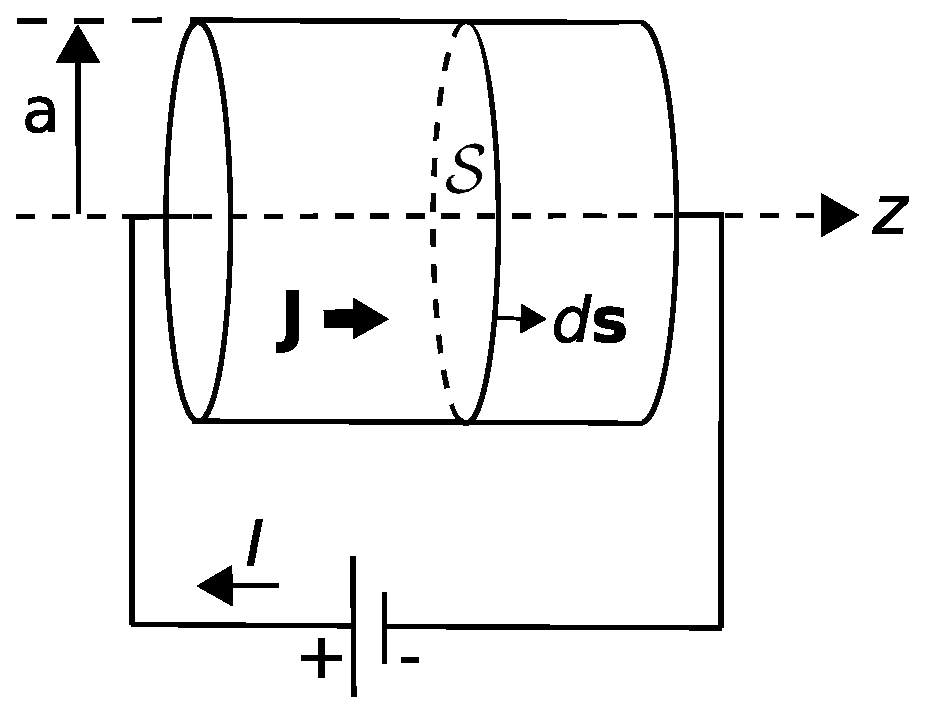
\includegraphics[width=2in]{modules/m0101_fMatEx1.eps}
% https://commons.wikimedia.org/wiki/File:M0101_fMatEx1.svg
}}{A three dimensional section of wire with radius a lies on its side centered on the z-axis. It is connected to a battery, with the positive end connected at the left side and the negative end connected at the right side of the cylinder. A cross-section is labeled S. From the cross-section extends a vector d bold s. Current shown flowing clockwise and current density shown going left to right through the cylinder.}
\end{center} 
\centerline{\scriptsize 
\copyright~\hyperref[m0101_fMatEx1_Credit]{K.\ Kikkeri} 
\href{https://creativecommons.org/licenses/by-sa/4.0/}{CC BY~SA 4.0} 
} 
\caption{
\label{m0101_fMatEx1}
Net current $I$ and current density ${\bf J}$ in a wire of circular cross-section. 
}
\end{figure}
\end{example}

%%%%%%%%%%%%%%%%%%%%%%%%%%%%%%%%%%%%%%%%%%%%%%%%%%%%%%%%%%%

{\bf Additional Reading:}
\begin{itemize}
\item ``\href{https://en.wikipedia.org/wiki/Electric_current}{Electric current}'' on Wikipedia.
\item ``\href{https://en.wikipedia.org/wiki/Current_density}{Current density}'' on Wikipedia.
\end{itemize}

\index{current density|)}







